\section{Introduction}
\label{sec:intro}

In this {\it Earth System Modeling Framework (ESMF) Architecture Document} we describe 
the main design features that will enable us to achieve interoperability, ease of 
use, performance portability, and reuse for climate, weather, and data assimilation
applications.  Our goal is to create a software system capable of satisfying
the extensive functional requirements laid out in the {\it ESMF 
Requirements Document}, while retaining in its design a measure of intuitiveness
and simplicity. 

We define a framework as a structured collection of software building blocks 
that can be used or customized to develop model components, assemble them into an 
application, and run the application.  Unlike a software library, in a framework some
software elements are partly defined or unimplemented.  For example, a framework
may require that a gridded model provide a {\tt GetGrid} method, and specify 
a format for describing the grid, but leave the implementation of the method up
to the framework user.  This relatively non-intrusive standardization enables 
different model components to interoperate with each other, and to use fully
complete, general methods provided by the framework (in this case, perhaps a 
{\tt Regrid} method).

The functional split between developing and combining components is the
foremost feature of the ESMF architecture.  The simplest view of the ESMF 
is that it consists of an {\it infrastructure} of utilities and data 
structures for building model components and a {\it superstructure} for coupling 
and running them.  User-provided components fit between these 
layers like the filling in a sandwich.  Each successively higher layer builds
on elements of the one below it.  Utilities such as communication
primitives, logging and profiling tools are used in methods that
manipulate field and grid data structures.  These data structures may in 
turn be integrated into user-supplied components, or they may simply 
help to wrap a component's native data structures in order to provide 
a standard interface.  The superstructure provides a systematic approach to 
sequencing and synchronizing user-supplied components.  The main layers
in the ESMF architecture are shown in Figure~\ref{fig:sandwich}.  

\begin{figure}
\label{fig:sandwich}
\scalebox{0.7}{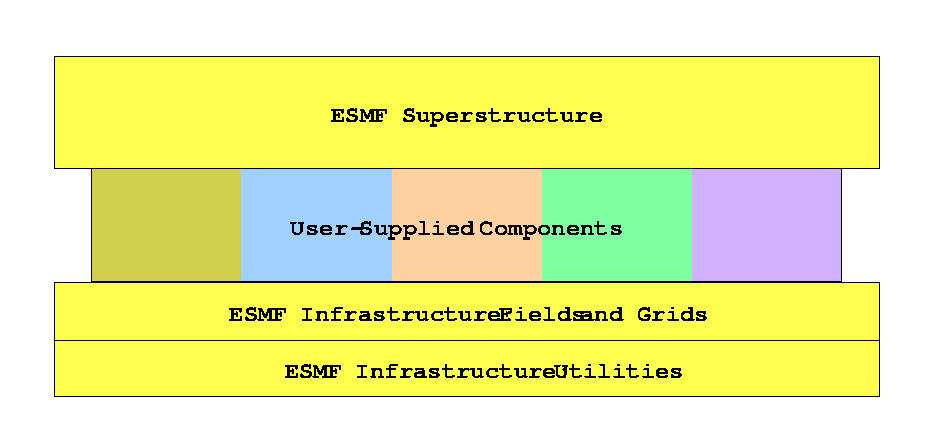
\includegraphics{Sandwich.eps}}
\caption[{ESMF Architecture}]{The simplest view of the ESMF architecture
is that it consists of an infrastructure for developing components and 
a superstructure for assembling applications.}
\end{figure}

The document is organized as follows.  Section~\ref{sec:shortscope} is a summary of the 
scope and motivating requirements of the ESMF, which are explained in more detail in 
the {\it ESMF Requirements Document}.  In Section~\ref{sec:archbackground}, 
we examine existing frameworks within our community and how they have motivated
and influenced ESMF design.  
Section~\ref{sec:strategies} describes how ESMF relates to several
major design paradigms.
Sections~\ref{sec:superclasses},~\ref{sec:fieldclasses}, and
\ref{sec:utilclasses} contain descriptions of the 
major classes in the framework, their structure, their relationships to each other, 
and the sequence of events for key interactions.  Section~\ref{sec:fwdesign}, {\it 
Framework-Wide Design Elements}, describes in detail the conventions and behavior
that we wish to apply across the ESMF software.  Section~\ref{sec:glos} is a 
glossary of terms.








